\section{Note compass }
Why is the music scale irregular? Why are there black and white keys in the piano, distributed in such a peculiar pattern? Why do we have a scale with tones and semitones? More deeply, how are notes grouped into families? What role do they play within such families? And more philosophically, what turns a sequence of notes into music? The answers may be buried in musical tradition and notation, which may appear obscure and confusing. This Note Compass can help us to orient ourselves and to find the logic behind it.

Underlying all the Western music tradition is the idea that the available notes -- when examined from low to high -- repeat cyclically. Aside from acoustic considerations, the octave is the period of repetition of notes, named as such because we traditionally choose to have seven notes on each cycle (so the eighth is again the first, in circle). We call such a periodic selection of notes a scale.

A fundamental property of the scale in Western tradition is that it is generated by a single interval (up to octave windings around the circle). This generating interval is a favored distance between some notes that appears repeatedly, and depending on its size it may result that the seven notes are not evenly distributed on the cycle\footnote{We cannot know for sure whether the scale was historically invented on the basis of this property, because it is logically equivalent to other musically relevant properties.}. To perform the scale generation we start with a first note and add the generating interval to get the second note, then we repeat this procedure until we get 7 notes\footnote{In order to experiment with other generating intervals and scales with less or more notes, see the `Scale theory'
section in the Scale Lab exhibit.}. This generating interval is called perfect fifth, because classically it is the distance between the first and fifth notes in the scale (four steps).

The generation property as such is independent of acoustics and does not prescribe the actual size of the generating fifth. But music tradition has favored a consonant interval. In the twelve-note system, which is a robust and practical simplification of the traditional notation system, the approach is to take a fifth interval of 7/12 of the size of the octave\footnote{An octave is acoustically associated to the interval between a frequency f and its double 2f. Normalizing the size of the octave to the log-frequency 1 = log2(2), the just tuned fifth of frequency ratio 3:2  has size log2(3/2)=0.58496 which is quite close to 7/12=0.58333, within a 0.16\% of difference.}. This means that the intervals between our seven notes come in multiples of the basic unit of 1/12 of the octave.

Graphically, we can think of the octave cycle as a circle, and the basic units of 1/12 length as the vertices of a dodecagon. The interval of the fifth is a jump of 7 basic units. If we join all the twelve fifth intervals (separated by 7/12 of the circle), we obtain a 12-pointed star. Our scale is then a selection of 7 out of the 12 points on the star, joined by the edges in a chain of fifths.

Thereby we will see that some points of the scale are adjacent (at distance of 1 unit) and others  leave  a gap of distance 2 (skipping over points which are not in the scale). By their arithmetic properties, it is impossible to distribute 7 out of  12 points evenly on the dodecagon, but the notes of our scale are distributed as evenly as possible. We find that there are always five major steps (2 units, also called tone) and two minor steps (1 unit, called semitone). The minor steps are separated by groups of two and three major steps, respectively. This scale is called the diatonic scale. If we account for the beginning and ending of the scale we end up with one of the following patterns (called modes), that receive Greek names:

\begin{center}
\begin{tabular}{rl}
	2 , 2 , 1 , 2 , 2 , 2 , 1 & Ionian (major) \\
	2 , 1 , 2 , 2 , 2 , 1 , 2 & Dorian \\
	1 , 2 , 2 , 2 , 1 , 2 , 2 & Phrygian \\
	2 , 2 , 2 , 1 , 2 , 2 , 1 & Lydian \\
	2 , 2 , 1 , 2 , 2 , 1 , 2 & Mixolydian \\
	2 , 1 , 2 , 2 , 1 , 2 , 2 & Aeolian (minor) \\
	1 , 2 , 2 , 1 , 2 , 2 , 2 & Locrian \\
\end{tabular}
\end{center}
Note that all the modes are in cyclic permutation of each other, that is, taking each time the first item and placing it on the end. With this model, to create any concrete mode you only need to choose one of the 12 points (tonic note), and one of the 7 step patterns that you want to use. This gives you 12 · 7 = 84 possibilities. It is important to observe that the mode is not just the set of 7 notes, it is also their order and starting point that matters.

The Note Compass allows you to visualize the 84 different possible diatonic modes. The instrument consists of two concentric disks. The foreground rotating 12-pointed star represents the 12 notes in an octave. The background plate is divided into sectors that allow to select the notes. Notes on the star that lie on a colored sector are part of the mode, notes that lie on a gray sector are not. The multicolor keyboard of the tone compass app has only the keys for the notes in the scale, and not the others.

How do these arithmetic and combinatorial properties relate to music? First of all, in order the play the notes you need to assign a pitch (or pitch class) to each of the 12 vertices of the star. The precise pitch is a tuning or intonation issue that we leave aside here, but we just remark that pitch is just one attribute of the performance of a note.


Secondly, the notes of a mode behave as a family, and interact with one another and provide a unique character to each family member. The first note in a mode is called tonic, and it serves as an anchor for the entire family. When a musical piece is said to be in C-major, then it is the note C which serves as the tonic. In a piece in C-minor the same note serves as the tonic, but it has a different character. And of course, the same note C can serve in different roles and can have different characters in other modes. Thus, its order position inside the mode and the relation to the major and minor steps are also other attributes of a note that refer to its function inside the logic of the composition.

In view of these attributes, there are three ways to refer to a note:

\begin{enumerate}

\item Latin note names A, B, C, D, E, F, G (possibly with sharps or flats attached to them) indicate the pitch heights to be played. It is fixed as soon as your instrument is tuned. For instance, in modern equal temperament tuning, the middle A is 440 Hz. Note names appear in the twelve needles of the turnable star-shaped dodecagon.

\item Arabic numerals 1, 2, 3, 4, 5, 6, 7, (8 = 1) designate their position (scale degree) in the scale in ascending order. Scale degree 1 refers to the tonic note musically governing the collection of the seven scale degrees. Each numeral corresponds to one of the ``rainbow''-colored segments in the outer disk of the tone compass (1 = red, 2 = orange, 3 = yellow, 4 = light green, 5 = dark green, 6 = dark blue, 7 = violet). In any configuration of the compass there are precisely seven of the 12 note-name-needles pointing into these seven colored segments and thereby to the seven scale degrees 1, 2, 3, 4, 5, 6, 7.

\item Syllables do, re, mi, fa, so, la, ti designate the different characters of the seven notes, arising from the specific locations with respect to the two minor steps in the step interval pattern. The minor steps (1 semitone) are always located between mi-fa and between ti-do. One may think of a mode as a little society of notes, where a unique character may be attributed to each note. On the Note compass, the seven syllables appear in the little subdivisions of each colored segment in the (counter-clockwise) order fa - do - so - re - la - mi - ti. In any configuration of the compass the seven active needles (pointing into colored segments) also point precisely to one of the seven syllables each.

\end{enumerate}

Note that the latin note names are
\begin{center}
C, C$\sharp$/D$\flat$, D, D$\sharp$/E$\flat$, E, F, F$\sharp$/G$\flat$, G, G$\sharp$/A$\flat$, A, A$\sharp$/B$\flat$, B.
\end{center}
The notation is essentially based on the diatonic scale, and it is anchored in one particular family of modes whose notes are named  by the single letters  A, B, C, D, E, F, G. They correspond to the white keys of the piano. All other  notes have accidentals $\sharp$ (sharps) or $\flat$ (flats) attached to their  names. A$\sharp$ is meant to be higher than A,  B$\flat$ is meant to be lower than B. The amount of alteration is the difference between the major and the minor step, and in the twelve-note system, A$\sharp$ and B$\flat$ are identified and located on the same needle of the star.

The seven notes of any diatonic mode are graphically represented on seven successive height degrees of the musical staff. Their note names always run through all the seven latin names A, B, C, D, E, F, G (possibly supplemented with either sharps $\sharp$ or flats $\flat$ so that we don't have pairs like A and A$\sharp$ in the same mode). The locations of the major and minor steps are graphically not explicitly shown, musicians know them implicitly from the clefs.

This is a tribute to historical tradition, to the fact that all modes are instances and, at the same time, alterations of one single scale (that today we call C-Major).

Let us see an example of the Note Compass working. Start with the most usual scale: C-Major (or C-Ionian). Point the needle with the C pitch note to the red sector pointing to syllabe do. We have this familiar concordance:

C -> (1, do), D -> (2, re), E -> (3, mi), F -> (4, fa) , G -> (5,so), A -> (6, la), B -> (7, ti)

Observe that the active needles are (from the 1st to 7th sectors) arranged in steps  2,2,1,2,2,2,1 (Ionian mode). The minor step (1 semitone) is when two consecutive needles are active.

Now move the star one elementary rotation in the counter-clockwise direction. The B-needle pointing to (7, ti) leaves the violet-colored segment and points into the gray segment between the violet and the red one. It is no longer an active note of the chosen mode. Instead the B$\flat$-needle enters from a previously gray position between the dark blue and violet segments into the violet segment and points at the syllable fa. The minor step (ti-do) between B and C is transformed into a major step (fa-so) between B$\flat$ and C and the major step (la-ti) between A and B is transformed into a minor step (mi-fa) between A and B$\flat$. The resulting step interval pattern is 2,2,1,2,2,1,2 (Mixolydian mode).

It is crucial that with each elementary rotation only one needle gets de-selected and one (adjacent to it) gets selected, thus only one note is altered in the scale. This fact comes from the particular irregularity of the step pattern of the diatonic scale. Mathematically, it is a cyclic permutation of the step pattern that can also be obtained by switching adjacent steps (a transposition). Here is an illustration of this peculiarity: If we rotate the name of our exhibition lalalab four letters to the left, we obtain lablala. If we exchange its last two letters, we obtain lalalba, which obviously is different from lablala. Applying, however, these two transformations to the Ionian step interval pattern 2212221, we obtain 2212212 in both cases.

This property is reflected in how musicians use the key signature in the staff to notate the mode, namely by adding just one flat or sharp at a time.

Finally, a few remarks on the nomenclature in different European traditions, that can be a source of confusion: Firstly, in German-speaking countries, the notes B and Bb are called H and B, respectively. This comes etymologically from the b quadratum and the b rotundum and it has stuck into tradition. Secondly, in most Romance and Slavic languages, the syllables do, re, mi fa, sol, la, si have been hijacked to replace the roman letters C, D, E, F, G, A, B in their role of note names. This use can be traced back to around 1600 in France, although the six syllables ut, re, mi, fa, sol, la appear much earlier, around 1000 AD with Guido of Arezzo.

Despite of differences in naming and teaching traditions musicians are aware of the importance of all three specifications of a note (pitch height, scale degree, modal character). The tone compass conveys the nature of their interdependence. For the music lover it might be enlightening to understand how music notation and practice subtly encapsulate tradition, perception and arithmetic insight.

\begin{figure}[hp]
\centering
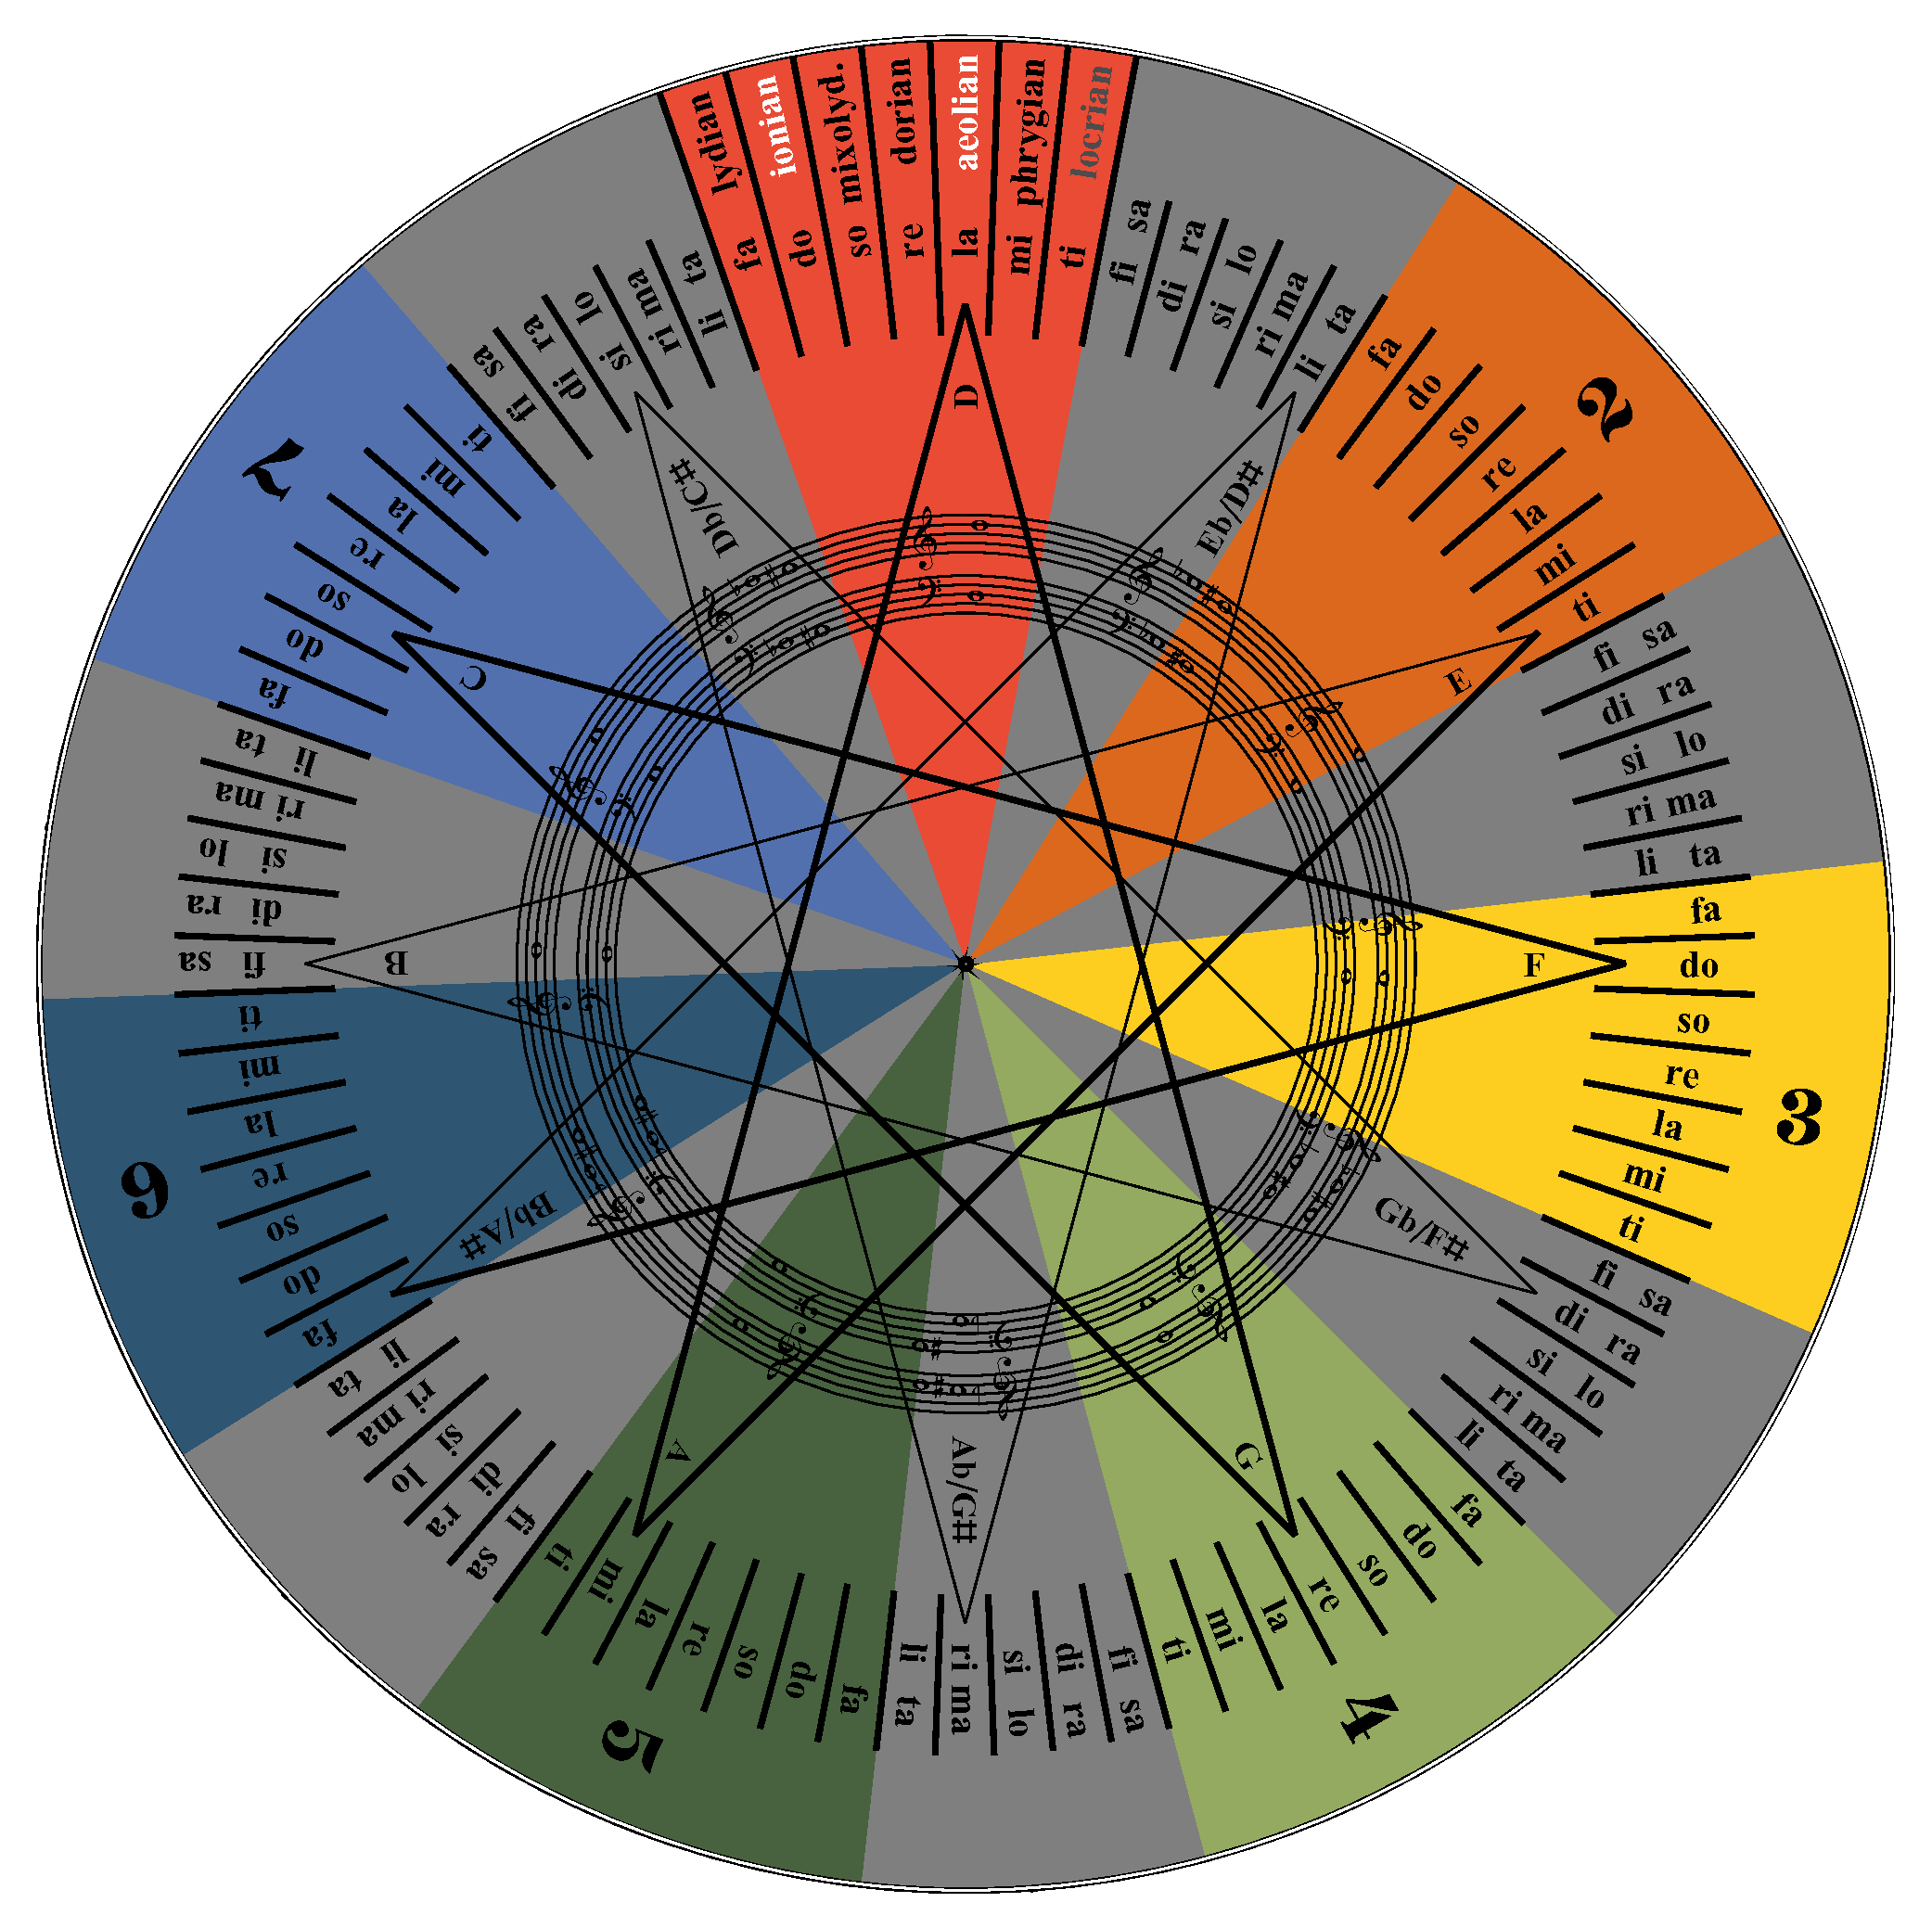
\includegraphics[width=0.95\textwidth]{NoteCompass_1}
\caption*{Note Compass displaying D-Aeolian. The thicker lines on the star mark the chain of fifth intervals in the scale.}
\end{figure}


\begin{sectcredits}
\item[Authors of the exhibit:] Thomas Noll (conception) and Daniel Ramos for IMAGINARY (implementation).
\item[Text:] Thomas Noll and Daniel Ramos.
\end{sectcredits}
